\section{Resultados}
\begin{table}[h!]
    \centering
    \begin{tabular}{|c|c|c|}
    \hline
    Puntos & Iteraciones & Tiempo (ms)\\
    \hline
    4 & 6 & 622600\\
    \hline
    8 & 28 & 144300\\
    \hline
    16 &120 & 129900\\
    \hline
    32 &496 & 233000\\
    \hline
    64 & 2016 & 1754700\\
    \hline
    128 & 8128 & 1498600\\
    \hline
    256 & 32640 & 7091000\\
    \hline
    512 & 130816 & 15373200\\
    \hline
    1024 & 523776 & 15469900\\
    \hline
    2048 & 2096128 & 21580900\\
    \hline
    4096 & 8386560 & 56996600\\
    \hline
    8192 & 33550336 & 459652300\\
    \hline
    16384 & 134209536 & 1083541700\\
    \hline
   32768 & 536854528 & 4046464200\\
    \hline
    65536 & 2147450880 & 22597086800\\
    \hline
    131072 & 8589869056 & 135702551400\\
    \hline
    262144 & 34359607296 & 802027289500\\
    \hline
    \end{tabular}
    \caption{Resultados fuerza bruta}
    \label{tab:bruteT}
\end{table}
\begin{figure}[h!]
    \centering
    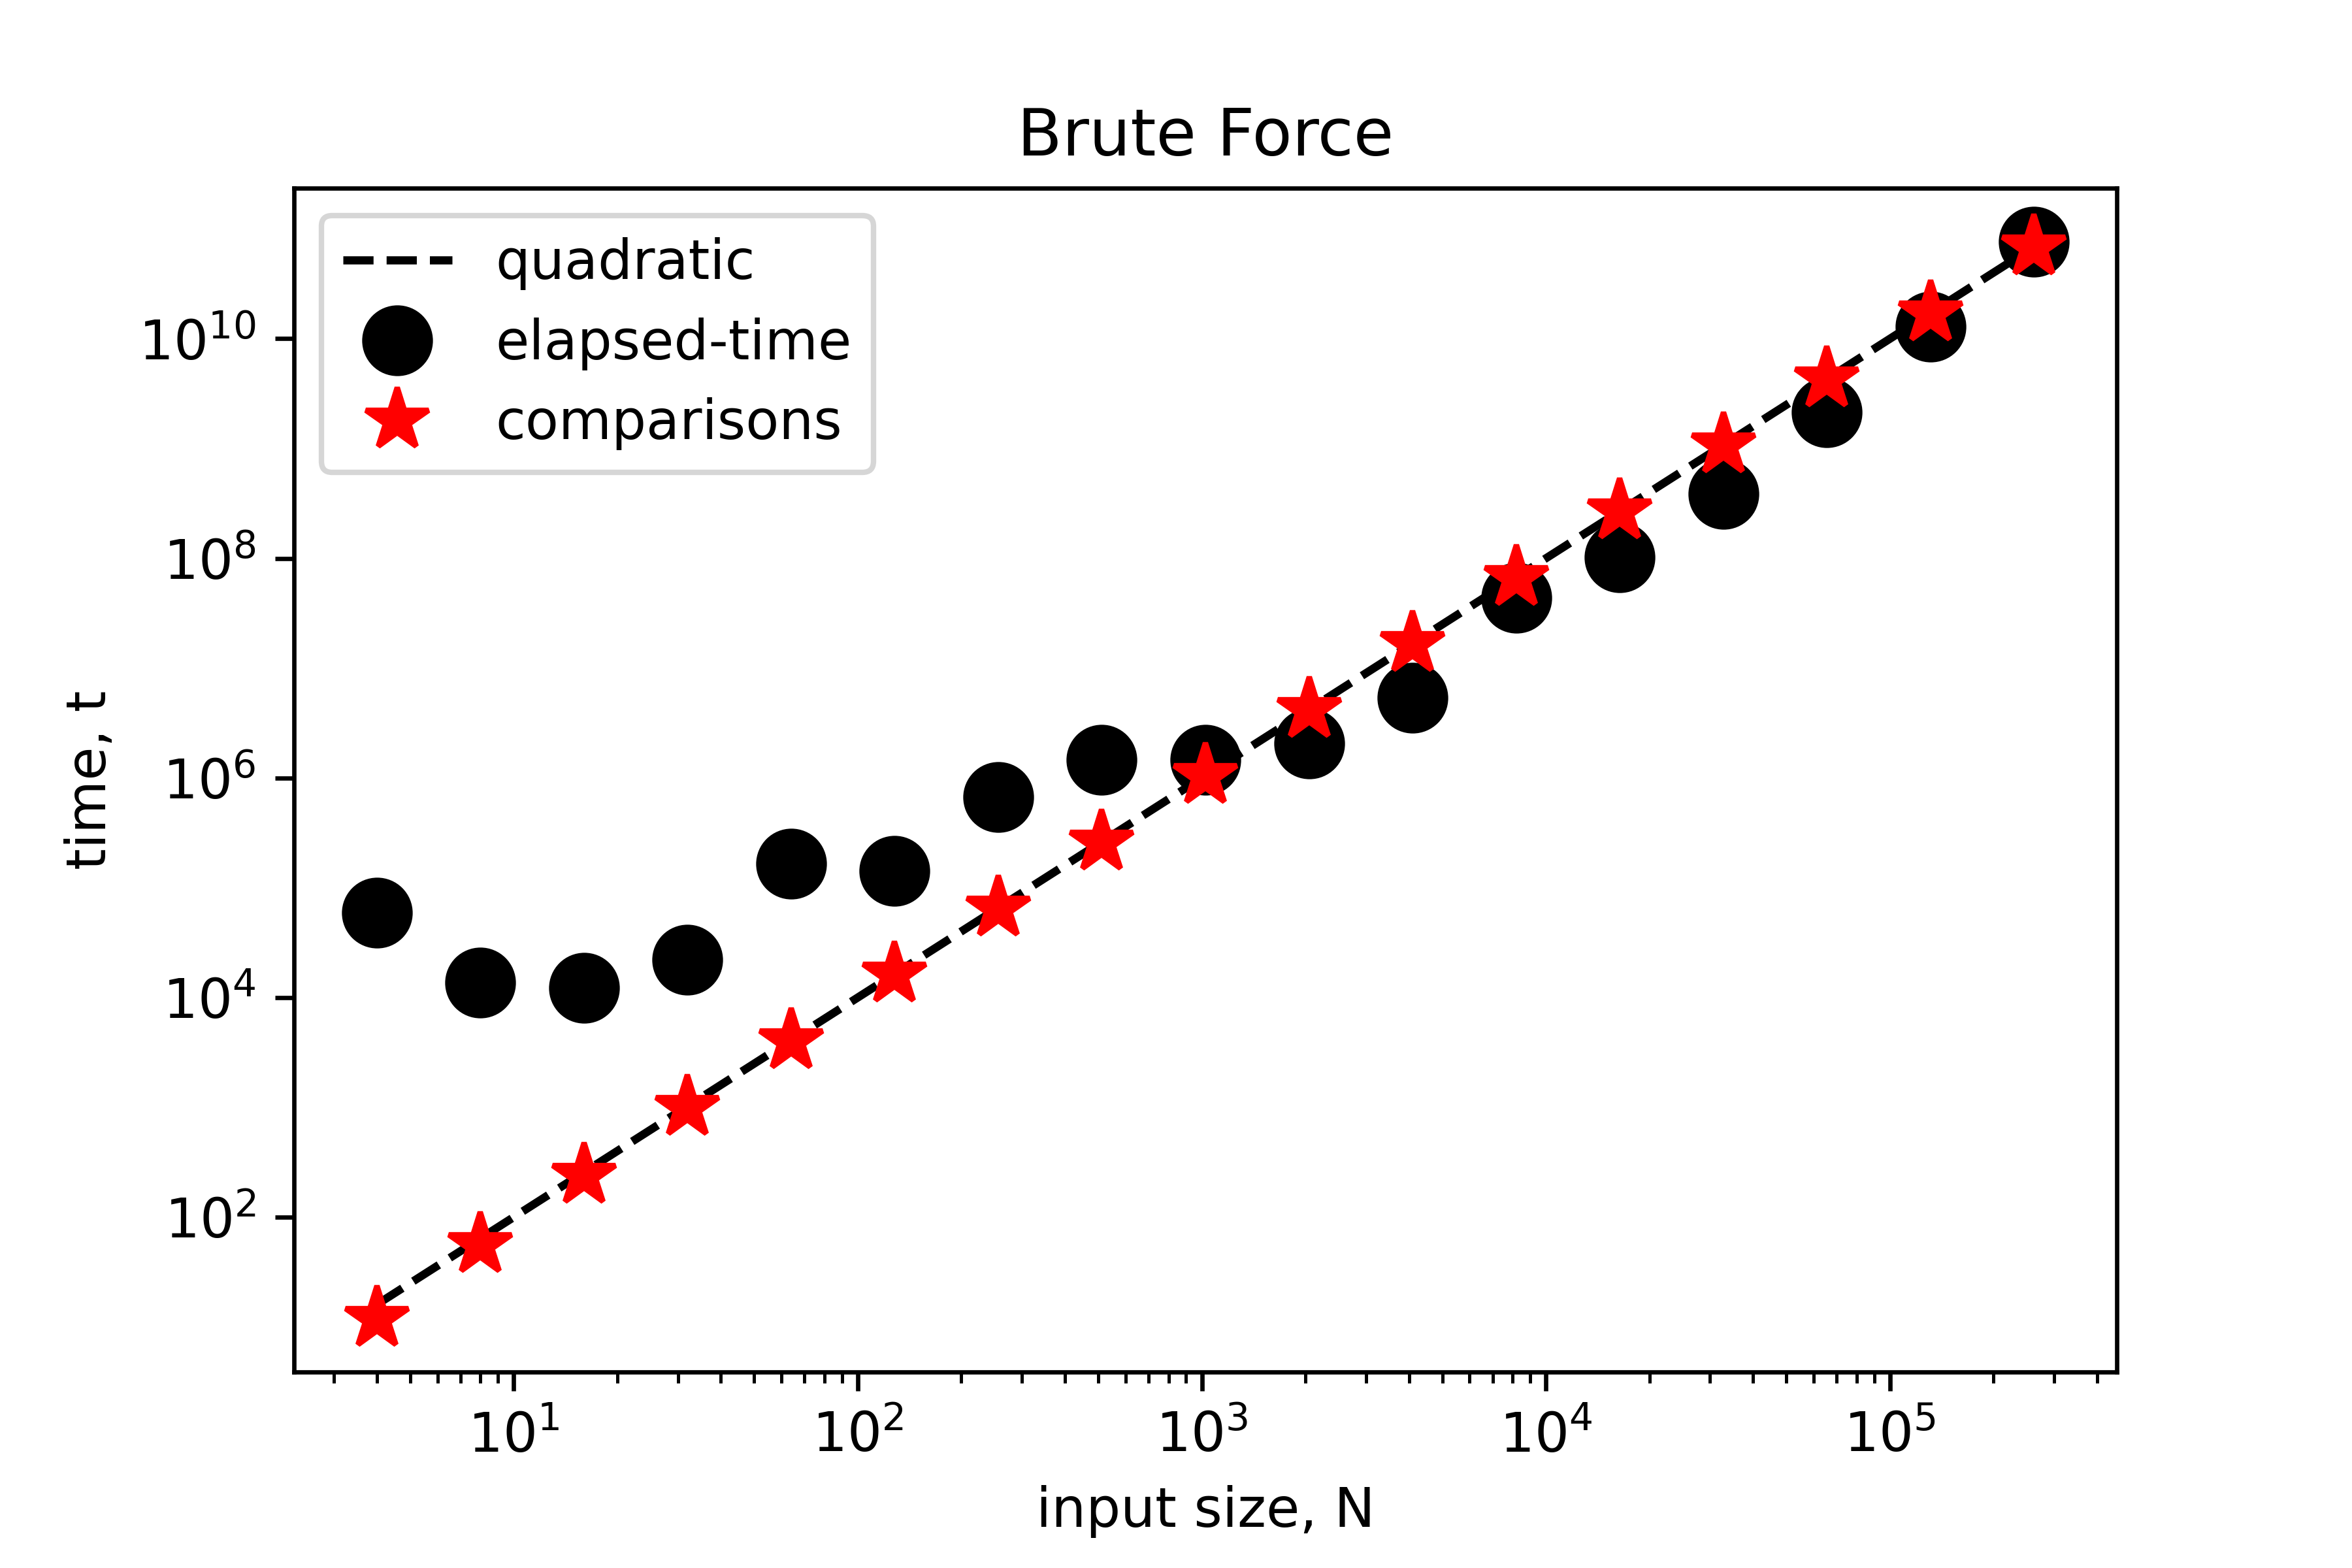
\includegraphics[scale=0.8, center]{images/brute.png}
    \caption{ Resultados algoritmo iterativo}
    \label{iterG}
\end{figure}
\begin{table}[h!]
    \centering
    \begin{tabular}{|c|c|c|}
    \hline
    Puntos & Iteraciones & Tiempo (ms)\\
    \hline
    4 & 3 & 10487775\\
    \hline
    8 & 16 & 758975\\
    \hline
    16 & 72 & 661400\\
    \hline
    32 & 240 & 486275\\
    \hline
    64 & 992 & 601150\\
    \hline
    128 & 4032 & 1163550\\
    \hline
    256 & 16256 & 2936900\\
    \hline
    512 & 65280 & 4203275\\
    \hline
    1024 & 261632 & 3493450\\
    \hline
    2048 & 1047552 & 7773700\\
    \hline
    4096 & 4192256 & 25683525\\
    \hline
    8192 & 16773120 & 102718075\\
    \hline
    16384 & 67100672 & 445447950\\
    \hline
   32768 & 268419072 & 1575060025\\
    \hline
    65536 & 1073709056 & 6736732150\\
    \hline
    131072 & 4294901760 & 33748572725\\
    \hline
    262144 & 17179738112 & 270556875925\\
    \hline
    \end{tabular}
    \caption{Resultados divide and conquer}
    \label{tab:divideT}
\end{table}
\begin{figure}[h!]
    \centering
    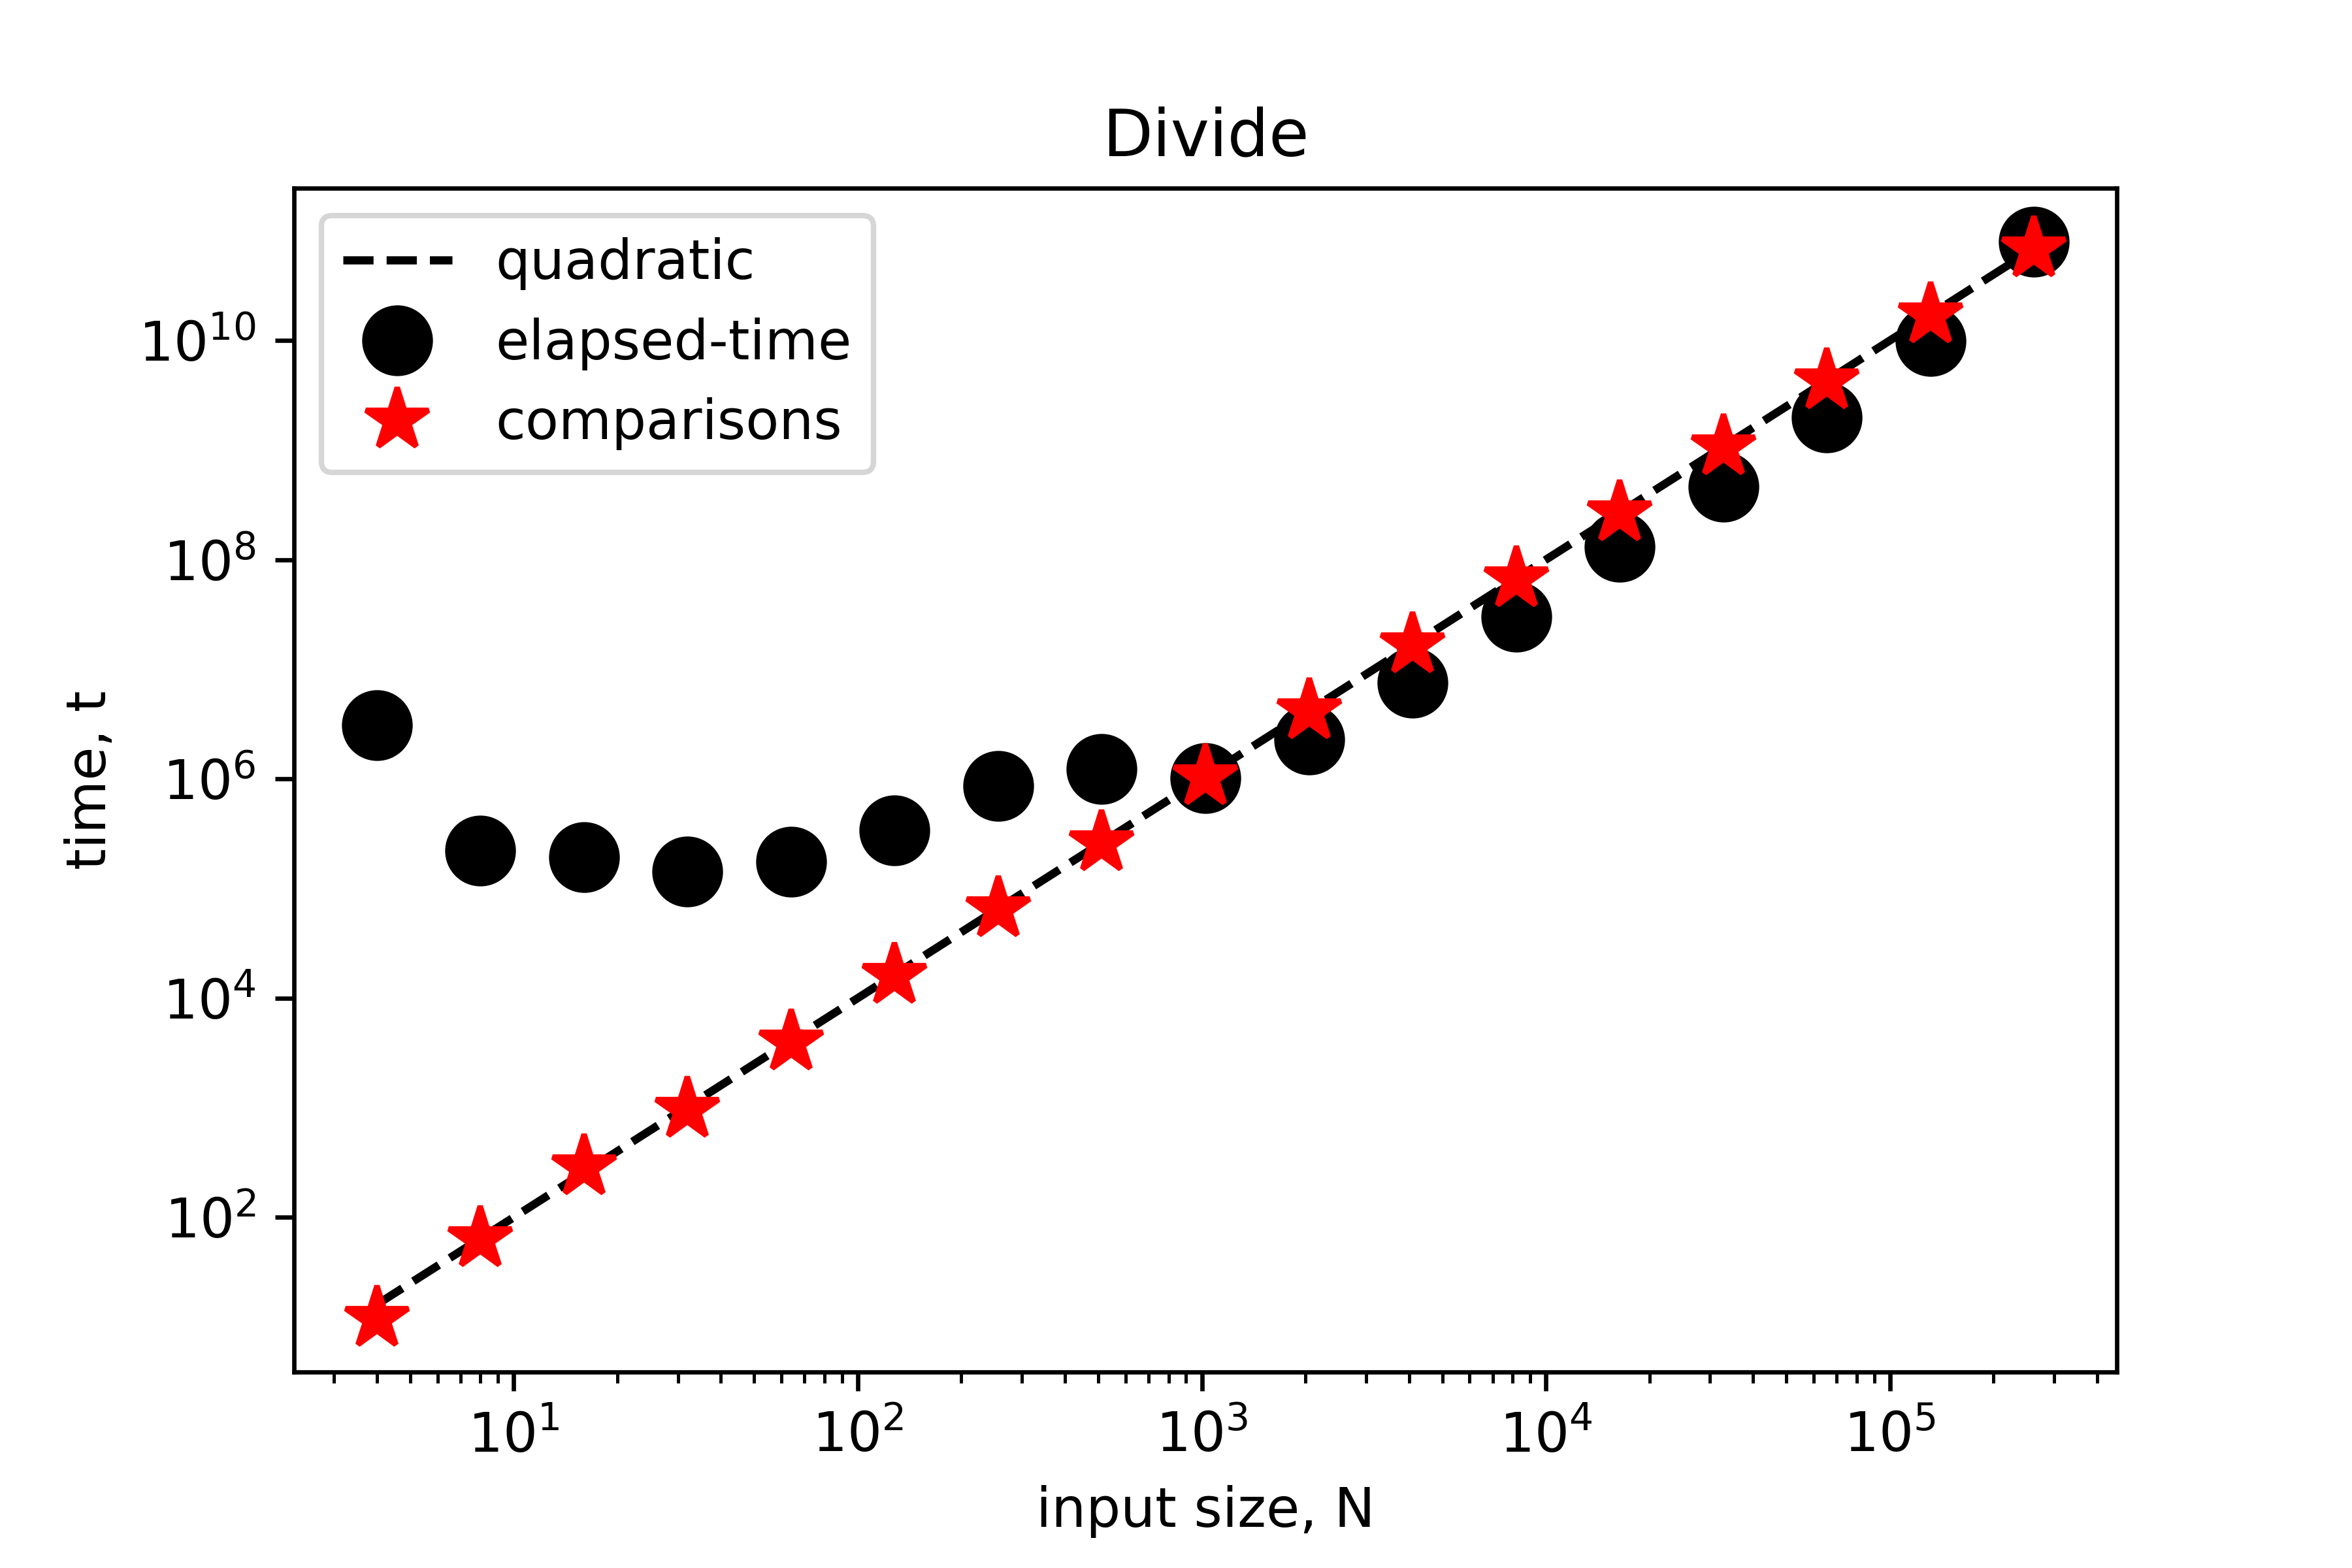
\includegraphics[scale=0.8, center]{images/divide.png}
    \caption{Resultados algoritmo divide and conquer}
    \label{divG}
\end{figure}
\FloatBarrier